\documentclass[numbers=endperiod]{scrartcl}
%test

%\usepackage{fontspec}
%\setmainfont{Calibri}
\renewcommand{\familydefault}{\sfdefault}


\usepackage{geometry}
\geometry{
	a4paper,
	total={170mm,257mm},
	left=20mm,
	right=20mm,
	top=20mm,
	bottom=39mm
}

\usepackage{fancyhdr}
\usepackage{lastpage}
\usepackage{graphicx}
\usepackage{caption}
\usepackage{blindtext}
\usepackage{enumitem}
\usepackage[hidelinks]{hyperref}
\usepackage{MnSymbol}%
\usepackage[dutch]{babel}

%Bibliography
\usepackage[style=ieee]{biblatex}
\begin{filecontents}{test.bib}
	@ONLINE{SER:2013:Online,
		author = {{Sociaal-Economische Raad}},
		title = {Energieakkoord \uppercase{SER}},
		year = {2013},
		url = {http://www.energieakkoordser.nl/},
		urldate = {2016-11-24}
	}
	@ONLINE{Kavelbesluit:2015:Online,
		author = {{Ministerie van Economische Zaken, Ministerie van Infrastuctuur en Milieu}},
		title = {Ontwerpkavelbesluit \uppercase{II} windenergiegebied Borssele},
		year = {2015},
		url = {https://www.rvo.nl/sites/default/files/2015/08/DOMUS-\%2315108163-v1-Eindversie_Ontwerpkavelbesluit_II_windenergiegebied_Borssele__opgemaakte_pdf.pdf},
		urldate = {2016-11-22}
	}
	@BOOK{Grit:2015:Book,
		author = {Roel Grit},
		title = {Projectmanagement},
		publisher = "Noordhoff Uitgevers",
		address = "Houten, Groningen",
		year = {2015}
	}
	
\end{filecontents}
\bibliography{test.bib}

\usepackage[table]{xcolor}% http://ctan.org/pkg/xcolor
%\captionsetup{belowskip=1pt,aboveskip=0pt}


\graphicspath{ {./images/} }
\renewcommand{\figurename}{Figuur }
\renewcommand{\tablename}{Tabel }

\setlist{nosep,after=\vspace{2pt}} %For space after lists

\usepackage{xcolor}

\definecolor{hhs_theme_heading_1}{RGB}{26,104,169}
\definecolor{hhs_theme_heading_2}{RGB}{179,214,243}
\definecolor{hhs_theme_heading_3}{RGB}{170,183,52}

\addtokomafont{section}{\normalfont\Large}

\setkomafont{section}{\sectionheading}
\newcommand{\sectionheading}[1]{%
	\normalfont
	\Large%\sf\bf%
	\setlength{\fboxsep}{0cm}%already boxed
	\colorbox{hhs_theme_heading_1!80}{%
		\begin{minipage}{\linewidth}%
			\vspace*{6pt}%Space before
			\hspace*{4pt}
			\color{white}
			#1
			\vspace*{4pt}%Space after
		\end{minipage}%
		%\vspace*{-100pt}
}}

\newcommand{\sectionSmall}[1]{
	\vspace{-10pt}
	\section{#1}
	\vspace{-5pt}
}

\setkomafont{subsection}{\subsectionheading}
\newcommand{\subsectionheading}[1]{%
	\vspace{-10pt}
	\normalfont
	\Large
	\setlength{\fboxsep}{0cm}%already boxed
	\colorbox{hhs_theme_heading_2!80}{%
		\begin{minipage}{\linewidth}%
			\vspace*{4pt}%Space before
			\hspace*{2pt}
			#1
			\vspace*{4pt}%Space after
		\end{minipage}%
}}

\setkomafont{subsubsection}{\subsubsectionheading}
\newcommand{\subsubsectionheading}[1]{%
	\vspace{-15pt}
	
	\normalfont
	\noindent
	\begin{minipage}{\linewidth}%
		\vspace*{4pt}%Space before
		%\hspace*{-29pt}
		#1
		\vspace*{-10pt}
		\textcolor{hhs_theme_heading_1}{\rule{\textwidth}{1.5pt}}
		\vspace*{-15pt}%Space after
	\end{minipage}%
}
%end test



\DeclareGraphicsExtensions{.pdf,.png,.jpg}
\pagestyle{fancy}
%\fancyhf{}
%\rfoot{Pagina \thepage \hspace{1pt} van \pageref{LastPage}}

\setlength{\headheight}{35pt} 
\setlength{\footheight}{135pt} 


\fancyhead[L]{%\begin{minipage}[b]{0.65\linewidth}
	
\includegraphics[scale=0.4]{Logo.png}
	\fancyhead[C]{\vspace{-40pt}\textcolor{hhs_theme_heading_1}{\tiny In opdracht van: \\}
\includegraphics[scale=0.14]{rijkswaterstaat.jpg}}}
\fancyhead[R]{\slshape \leftmark}

\fancyfoot[L]{ 
	\tiny 2016-11-22\textunderscore PVA\textunderscore Ricardo-Molenaar\\\textunderscore Martijn-van-Essen\textunderscore Plan-van-Aanpak\textunderscore vA01
}
\fancyfoot[C]{	%\begin{flushleft}
	%\hspace{100pt}
	%\vspace*{0pt}
	\small Ricardo Molenaar \& Martijn van Essen\\
	PROENT\\
	vA02 \textbar 28-11-2016
	%\end{flushleft}
}	
\fancyfoot[R]{\vspace{0pt}\small \textbar Pagina \thepage \hspace{1pt} van \pageref{LastPage}\textbar}

\newcommand{\whitespace}{\vspace*{2 mm} \\}%Space between paragraphs
\newcommand{\moveup}{\vspace*{-7pt}}%Space between paragraphs
\newcommand{\toRomanNumber}[1]{\uppercase\expandafter{\romannumeral #1\relax}} %Create roman numerals

\newcommand{\tableref}[1]{\hyperref[table:#1]{tabel~\ref{table:#1}}}
\newcommand{\figureref}[1]{\hyperref[figure:#1]{tabel~\ref{figure:#1}}}


\renewcommand{\footrulewidth}{0.4pt}%

%\renewcommand{\labelitemi}{$\blacksquare$}


\title{Plan van Aanpak PROENT}
\date{18-11-2016}
\author{Martijn van Essen \& Ricardo Molenaar}

\usepackage{pdfpages}

\begin{document}
	%Title page
	\pagenumbering{gobble} %Turn off page numbers
	%\maketitle
	%\newgeometry{left=0cm,bottom=0cm}
	%\pagestyle{empty}
	%\vspace*{-3cm}
	%\includegraphics[scale=1]{cover.png}
	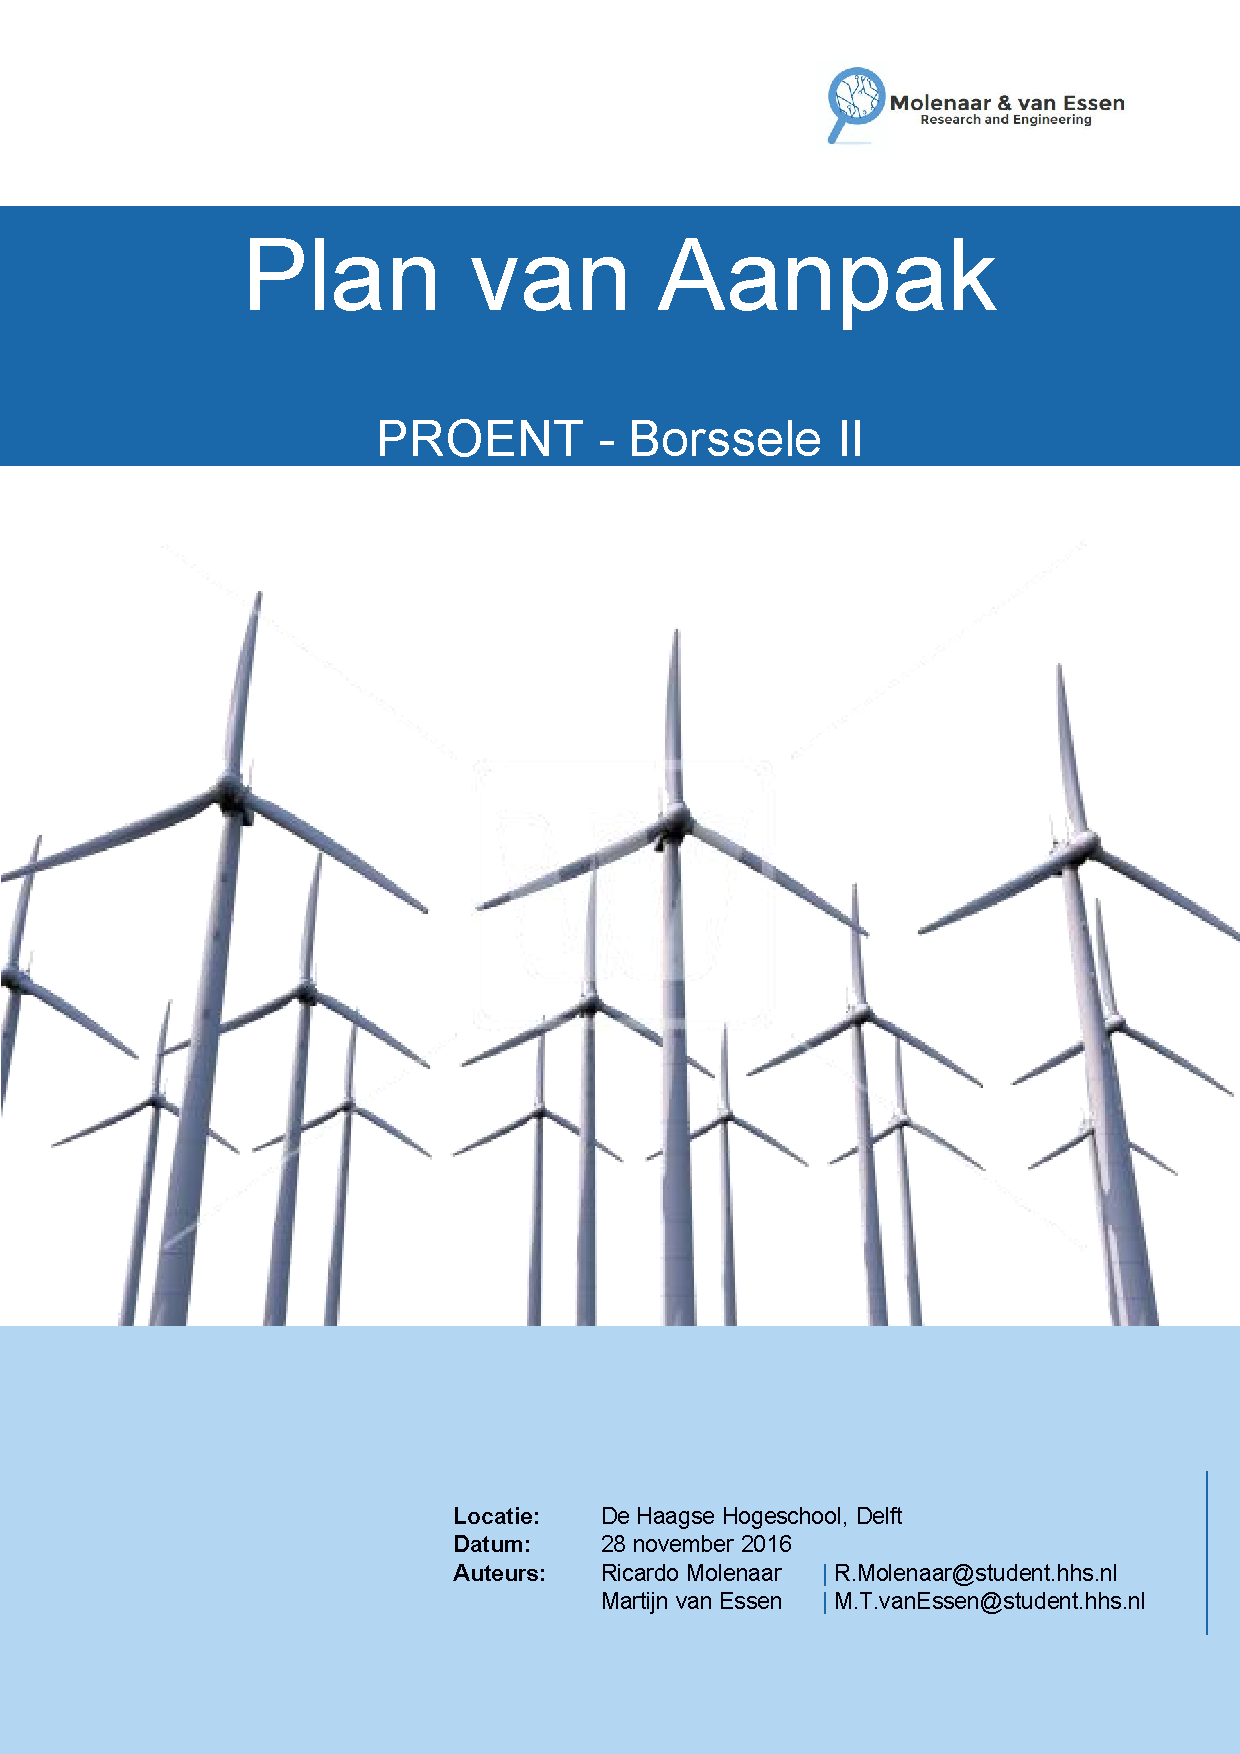
\includepdf{Cover}
	\newpage
	%\restoregeometry
	%End of title page
	
	%Versions page
	\pagenumbering{arabic} %Turn on page numbers
	\setcounter{secnumdepth}{0} %Turn off section numbering
	\sectionSmall{Versiebeheer}
	
	\begin{center}
		\begin{tabular}{| p{4cm} | l | p{7cm} | p{25mm} |}
			\hline
			
			\multicolumn{4}{|c|}{
				\cellcolor{hhs_theme_heading_2}
				Versiehistorie
			}  \\ \hline
			
			Versie 	& Datum 		& Wijzigingen 	& Auteur \\ \hline
			vA01 	& 22-11-2016 	& Lay out opstellen en indeling document    & M.T. van Essen\\ \hline
			vA02    & 25-11-2016    & Rapport tekstueel ingevuld                & R. Molenaar, M.T. van Essen \\ \hline
		\end{tabular}
	\end{center}
	\newpage
	%End of Versions Page
	
	%Table of contents
	\setcounter{tocdepth}{2}% 1 and 1.1 levels in table of content
	\tableofcontents
	\newpage
	%End of Table of contents
	
	\setcounter{secnumdepth}{3}%Turn on section numbering
	
	\sectionSmall{Projectachtergrond}
	In dit hoofdstuk worden de achtergronden van het project besproken. Hier wordt informatie gegeven over de achtergrond en algemene gegevens van het project.	
	\subsection{Naam}
	Voor dit project is de naam Windturbinepark Borsele II gekozen. PROENT is de projectcode waar deze opdracht deel van uitmaakt. Windpark Borssele II is de locatie waarvoor het ontwerp- en beheersplan geschreven zal worden.
	\subsection{Opdrachtgever}
	De opdrachtgever voor dit project is Rijkswaterstaat. Zij verdelen de kavels waarop de windparken gebouwd zullen worden aan de hand van verschillende ontwerp en beheersplannen, welke zij binnenkrijgen.
	\whitespace
	Rijkswaterstaat zal deze plannen beoordelen, maar zal verder geen actieve rol spelen in het aanleggen en beheren van het windpark.
	\subsection{Opdrachtnemer}
	De opdrachtnemer van dit project is ingenieursbureau Molenaar \& van Essen. Zij zijn verantwoordelijk voor het opleveren van een ontwerp en beheersplan bij Rijkswaterstaat.
	\subsection{Geschiedenis}
	In september 2013 zijn meer dan 40 organisaties akkoord gegegaan met het Energieakkoord \cite{SER:2013:Online}. In dit akkoord is afgesproken om in 2023 het aandeel van hernieuwbare energie met 16\% te verhogen.
	\whitespace
	Om dit plan te realiseren heeft Rijkswaterstaat een aantal kavels aangewezen voor de Nederlandse kust. Op deze kavels zullen windmolenparken gebouwd worden welke bijdragen aan het aandeel hernieuwbare energie.
	\subsection{Stakeholders}
	De opdrachtgever, Rijkswaterstaat, is bij dit project een grote belanghebbende. Zij zijn verantwoordelijk voor het bereiken van de eisen aan wind energie door de kavels op een goede manier te verdelen onder de bedrijven die deze willen exploiteren.
	\whitespace
	De Nederlandse overheid heeft ook belangen bij dit project. Door middel van dit project zijn zij in staat om aan de door de Europese Unie gestelde eisen aan duurzame energie te voldoen.
	\whitespace
	Verder heeft ook ingenieursbureau Molenaar \& van Essen. Zij kunnen in samenwerking met aannemer het windpark bouwen en vervolgens exploiteren.
	\subsection{Goedkeuring}
	De goedkeuring van het ontwerp en beheers plan zal door Rijkswaterstaat. Uit de verschillende inzendingen zullen zij het beste plan kiezen. Wanneer dit plan wordt goedgekeurd en uitgekozen zal de desbetreffende partij de rechten krijgen om dit plan uit te werken.
	\newpage
	
	\sectionSmall{Projectresultaat}
	In dit hoofdstuk wordt het doel van het project beschreven met hierbij de resulaten die hiermee behaald zullen worden.
	
	\subsection{Doelstelling}
	Om aan het energieakkoord te voldoen worden er windmolenparken op zee gebouwd. Het doel van dit project is om voor één van deze parken, namelijk Borssele II, een ontwerp en beheersplan te schrijven. Voor het schrijven van dit plan zal het projectteam onderzoek verrichten en aan de hand van hiervan zullen zij een ontwerp- en beheersplan schrijven.
	\whitespace
	Aan de hand van dit plan kan het windmolenpark gebouwd en vervolgens beheerd worden. Hierin wordt een voorstel voor een ontwerp van het kavel Borssele II. Naast dit ontwerp zal ook het beheersen van het park worden beschreven.
	
	\subsection{Resultaat}	
	Het resultaat van dit project is een ontwerp- en beheersplan. Tezamen vormt dit het projectplan. Dit plan zal worden ingediend bij Rijkswaterstaat waarna het beoordeeld zal worden. Daarnaast wordt er een projectarchief opgeleverd waarin alle gebruikte/opgestelde documentatie is opgenomen.
	\whitespace
	Wanneer het plan door Rijkswaterstaat als beste plan wordt ondervonden, zal er een vergunning worden verleend voor het realiseren van dit plan.
	%\newpage
	
	\sectionSmall{Projectactiviteiten}
	In dit hoofdstuk worden de activiteiten besproken welke in dit project plaats zullen vinden.
	\subsection{Besprekingen}
	Gedurende het project zullen een aantal gesprekken met de opdrachtgever plaatsvinden:
	\begin{itemize}
		\item projectweek 4: adviessessie Plan van Aanpak;
		\item lezingen van externe partijen: deze vormen een belangrijke basis voor het opstellen van het projectplan;
		\item nader in te plannen adviesgesprekken met de projectcoördinatoren.
	\end{itemize}
	\subsection{Documentatie}
	In dit project zal de volgende documentatie worden opgeleverd:
	\begin{itemize}
		\item Plan van Aanpak;
		\item Ontwerp- en Beheersplan; tezamen het projectplan.
	\end{itemize}
	
	\subsection{Bijeenkomsten}
	Binnen dit project vinden een aantal lezingen plaats vanuit de energietechniek sector. Deze lezingen zullen worden bijgewoond door de opdrachtnemer. Via deze lezingen wordt meer informatie verzameld over de wijze van ontwerpen en beheersen van een windturbinepark.
	\whitespace
	Naast deze lezingen zullen er ook twee locaties bezocht worden. Deze betreffen: Kabelfabriek Prysmian en windpark Westermeerwind.
	
	\sectionSmall{Projectgrenzen}
	Dit hoofdstuk bevat de afbakening van het project. De afbakening zal worden besproken aan de hand van de volgende twee punten:
	\begin{itemize}[noitemsep]
		\item hoe ver gaat het project;
		\item hoe breed gaat het project.
	\end{itemize}
	\subsection{Afbakening}
	Het project zal worden afgebakend aan de hand van de grensactiviteiten, het budget en het tijdsbestek wat beschikbaar is.
	\subsubsection{Grensactiviteiten}
	De volgende grensactiviteiten zijn bij dit project van toepassing:
	\begin{itemize}
		\item Ontwerp- en Beheersplan: wordt gerealiseerd;
		\item Realiseren windpark: wordt niet gerealiseerd;
		\item Beheersplan in werking stellen: wordt niet gerealiseerd.
	\end{itemize}
	\subsubsection{Tijdsbestek en budget}
	Dit project wordt uitgevoerd in een tijdsbestek van 9 weken. Het project start op 17 november 2016 en zal afgerond worden op 24 januari 2017.
	\whitespace
	Het project bestaat enkel uit het opleveren van rapportages. Aangezien hier geen kosten aan verbonden zijn, is er ook geen budget beschikbaar gesteld voor dit project.
	\subsection{Programma van Eisen}
	Het programma van eisen is opgesteld aan de hand van de eisen welke door Rijkswaterstaat aangeleverd zijn. Deze eisen zijn deels terug te vinden in het kavelbesluit Borssele II \cite{Kavelbesluit:2015:Online}. Verder zijn deze eisen met Rijkswaterstaat vastgesteld.
	\whitespace
	Hierbij worden de volgende elementen behandeld:
	\begin{itemize}[noitemsep]
		\item Randvoorwaarden;
		\item Eisen Ontwerp- en Beheersplan.
	\end{itemize}
	\subsubsection{Randvoorwaarden}
	De volgende randvoorwaarden zijn gesteld aan het kavel Borssele II:
	\begin{itemize}[noitemsep]
		\item het kavel moet tussen de 342 MW en 380 MW aan energie leveren;
		\item de windturbines moeten aangesloten worden op een 700 MW transformatorstation van TenneT;
		\item de windturbines bevinden zich volledig binnen de grenzen van het 63,5 km\textsuperscript{2} grootte gebied;
		\item de locatie voor het windmolenpark betreft Borsele kavel II;
		\item het windturbinepark wordt gebouwd vanuit een thuishaven: Vlissingen. Dit houdt in dat mens en materiaal
		vanuit deze haven naar de bouwlocatie heen en weer worden gebracht. Productie van de installaties
		of onderdelen daarvan vindt niet in de thuishaven plaats. Dit betekent dat iedereen en alles eerst naar
		de thuishaven getransporteerd moet worden voordat het naar de bouwlocatie gaat;
		\item de inrichting van het windpark is in overeenstemming met het kavelbesluit;
		\item een windmolen is opgebouwd uit de volgende componenten: een fundament, mast, rotorbladen, gondel met eventueel een overbrenging, de elektrische generator en de elektrische installatie;
		\item er moet een vergunning aanwezig zijn om het ontwerp- en beheersplan uit te voeren (de verantwoordelijkheid hiervoor ligt bij de opdrachtgever).
	\end{itemize}
	\subsubsection{Eisen Ontwerp- en Beheersplan}
	De volgende eisen zijn gesteld aan het ontwerp- en beheersplan:
	\begin{itemize}
		\item de realisatie dient op een zo kort mogelijke termijn plaats te vinden;
		\item de realisatie van het turbinepark dient door een externe partij te worden uitgevoerd;
		\item de windturbines worden 25 jaar geëxploiteerd (in het kader van de uitvoeringskosten van het beheersplan zal deze eis hierin mee moeten worden gewogen), waarna deze afhankelijk van de situatie al dan niet worden afgebroken;
		\item de risico's tijdens de bouw en beheer zijn zo laag mogelijk;
		\item het ontwerp, bouwen en beheren is conform de filosofie van duurzame ontwikkeling;
		\item het gekozen type turbine is onderbouwd;
		\item Molenaar \& van Essen bepaalt welke onderdelen van een windmolen door welke leverancier geleverd worden;
		\item naast de windmolens zelf moet er infrastructuur komen die ervoor zorgt dat de opgewekte elektriciteit naar het vaste land getransporteerd kan worden;
		\item voor het beheer moeten maatregelen getroffen worden opdat mens, materiaal en milieu veilig gesteld worden;
		\item er dient een grafische weergave van het windpark in het projectplan te worden opgenomen;
		\item de risico’s tijdens het beheer van de turbines en het windpark moeten in kaart worden gebracht, gekwantificeerd en gemanaged worden. Deze taak wordt overgedragen aan Molenaar \& van Essen;
		\item van elk risico wordt aangegeven hoe deze wordt vermeden, verminderd of overgedragen respectievelijk zelf gedragen wordt;
		\item de risico's, alsmede de afdekking hiervan, worden in het projectplan opgenomen;
		\item het projectplan is formeel van aard en er wordt gebruikgemaakt van betrouwbare bronnen. Daarnaast dienen de gebruikte documenten goed gearchiveerd te worden en een duidelijke naamgeving te krijgen. Zie het hoofdstuk kwaliteit voor de borging hiervan. 
	\end{itemize}
	
	\sectionSmall{Kwaliteit}
	Om te zorgen dat het projectresultaat van voldoende kwaliteit is, zal deze kwaliteit continu gemonitord worden. Hiervoor vinden controles plaats door de projectgroep en door de opdrachtgever.
	\subsection{Controle door de projectgroep}
	Om de kwaliteit van het project te waarborgen zal de projectgroep op de volgende punten letten:
	\subsubsection{Software}
	Om compatibiliteitsproblemen te voorkomen zullen de software-pakketten worden gebruikt zoals weergegven in \tableref{Software}.
	
	\begin{table}[h]
		\caption{Gebruikte software}\label{table:Software}
		
		\centering
		\begin{tabular}{ p{.3\textwidth} | p{.3\textwidth} }
			Software:	    & Gebruik:          \\ \hline
			ShareLaTeX   	& Tekstverwerking	\\
			MS Projects    	& Planning  		\\
		\end{tabular}
		
	\end{table}
	
	\subsubsection{Documentatie}
	Vanuit de opdrachtgever zijn richtlijnen aangeleverd voor stijl en naamgeving van documenten. Deze richtlijnen zullen door de projecgroep gehandhaafd worden. \cite{Grit:2015:Book}
	
	\subsection{Controle door de opdrachtgever}
	In de derde week van het project vindt er een overleg met de opdrachtgever plaats over het plan van aanpak. In dit gesprek zal een advies gegeven worden aan de projectgroep aan de hand van het plan van aanpak.
	\whitespace
	Na dit gesprek zal er geen controle meer plaatsvinden door de opdrachtgever tot aan het moment van het indienen van het ontwerp- en beheersplan.
	\subsection{Controle eindresultaat}
	Bij afronding van het project wordt het ontwerp- en beheersplan bij de opdrachtgever ingeleverd. Dit vormt zoals eerder genoemd het projectplan. Vervolgens zal een toetsing plaatsvinden over de kwaliteit van het document. 
	
	\sectionSmall{Projectorganisatie}
	In dit hoofdstuk is informatie te vinden over de projectgroep en organisatie van dit project.
	\subsection{Organisatie}
	Het gestelde project is aangenomen door ingenieursbureau Molenaar \& van Essen. Dit bedrijf bestaat uit
	twee werknemers welke beide aan dit project zullen werken. Informatie hier over is weergegeven in \tableref{Projectorganisatie}. 
	\begin{table}[h]
		\caption{Projectorganisatie}\label{table:Projectorganisatie}
		
		\centering
		\begin{tabular}{ p{.3\textwidth} | p{.32\textwidth} | p{.3\textwidth} }
			Naam: 				& Studentnummer:& E-mailadres \\ \hline
			Ricardo Molenaar 	& 15087506	 	& R.Molenaar@student.hhs.nl \\
			Martijn van Essen 	& 15086135		& M.T.vanEssen@student.hhs.nl \\
		\end{tabular}
		
	\end{table}
	\subsection{Contactmomenten}
	Aangezien de projectgroep slechts uit twee leden bestaat, zal veel communicatie direct gebeuren. Hiervoor zijn verder geen vergaderingen nodig aangezien de leden zeer regelmatig met elkaar in contact zijn. Dit zal per WhatsApp plaatsvinden. De gereserveerde dag hiervoor in de projectweken is vrijdag. 
	\whitespace
	De activiteiten binnen dit project zullen gelijktmatig verdeeld worden over de beschikbare tijd. Hierbij wordt de vrijdag als belangrijkste moment genomen omdat de projectleden op dit moment het meeste tijd beschikbaar hebben voor project.
	\whitespace
	Door de kleine samenstelling van de projectgroep is het ook niet relevant om een projectleider aan te wijzen. De taken zullen in overleg tussen de twee groepsleden verdeeld worden. Hierbij wordt in acht genomen dat beide projectleden een gelijke hoeveelheid werk (50\%) voor het project verzetten.
	
	\sectionSmall{Planning}
	In \tableref{Planning} is een planning voor het verloop van dit project weergegeven. Dit is een compacte weergave van de planning. Een uitgebreide planning is te raadplegen in \hyperref[sec:BijlageA]{bijlage A}.
	\begin{table}[h]
		\caption{Projectplanning}\label{table:Planning}
		\centering
		\begin{tabular}{| p{.3\textwidth} | p{.32\textwidth} | p{.3\textwidth} |}
			\hline \rowcolor{hhs_theme_heading_2}
			Item: 				& Geschat begin:& Deadline \\ \hline
			Plan van Aanpak 	& 17-11-2016 	& 28-11-2016 \\ \hline
			Projectplan		 	& 28-11-2016	& 16-1-2017 \\ \hline
			Procesverslag		& 9-1-2017		& 16-1-2017 \\ \hline
			Eindassessment		& 17-1-2017		& 24-1-2017 \\ \hline
		\end{tabular}
	\end{table}
	
	\newpage
	\printbibliography
	
	\newpage
	\setcounter{secnumdepth}{0}%Turn off section numbering
	\sectionSmall{Bijlagen}
	\whitespace
	\subsection{Bijlage A: Strokenplanning} \label{sec:BijlageA}
	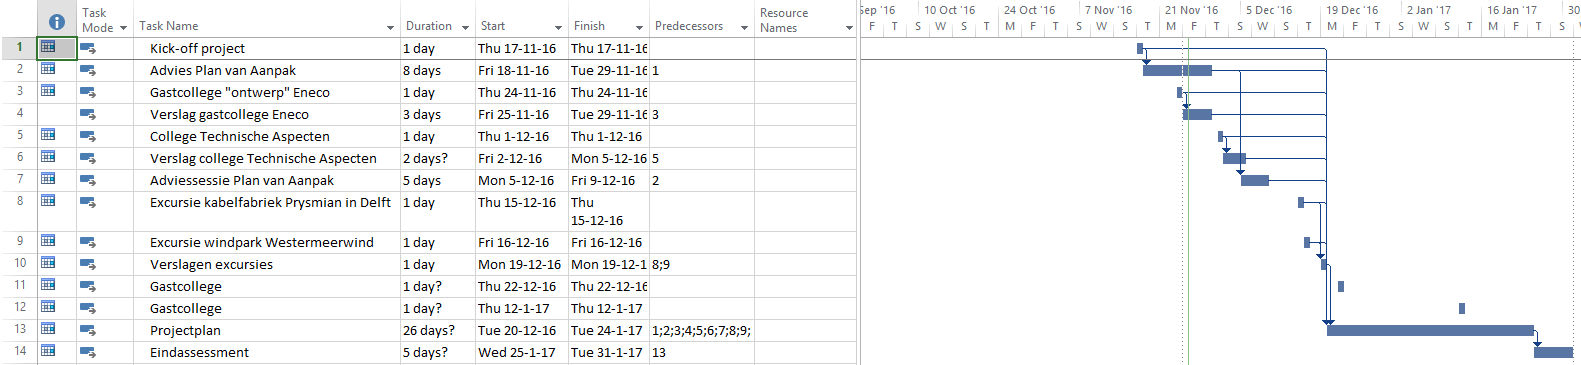
\includegraphics[angle=270,origin=c,scale=0.5]{Planning.PNG}	
\end{document}